\section{分组并行求解算法及其应用}
\begin{frame}
\frametitle{分组并行求解算法及其应用}
\begin{enumerate}
\item PGSolve: 分组并行算法
\item NS1L: 求n孤子-1 lump相互作用解的软件包
\item PGSolve 的求解效率
\end{enumerate}
\end{frame}

\subsection{PGSolve: 分组并行求解算法}
\begin{frame}
\frametitle{PGSolve: 分组并行求解算法}
\begin{figure}
\centering
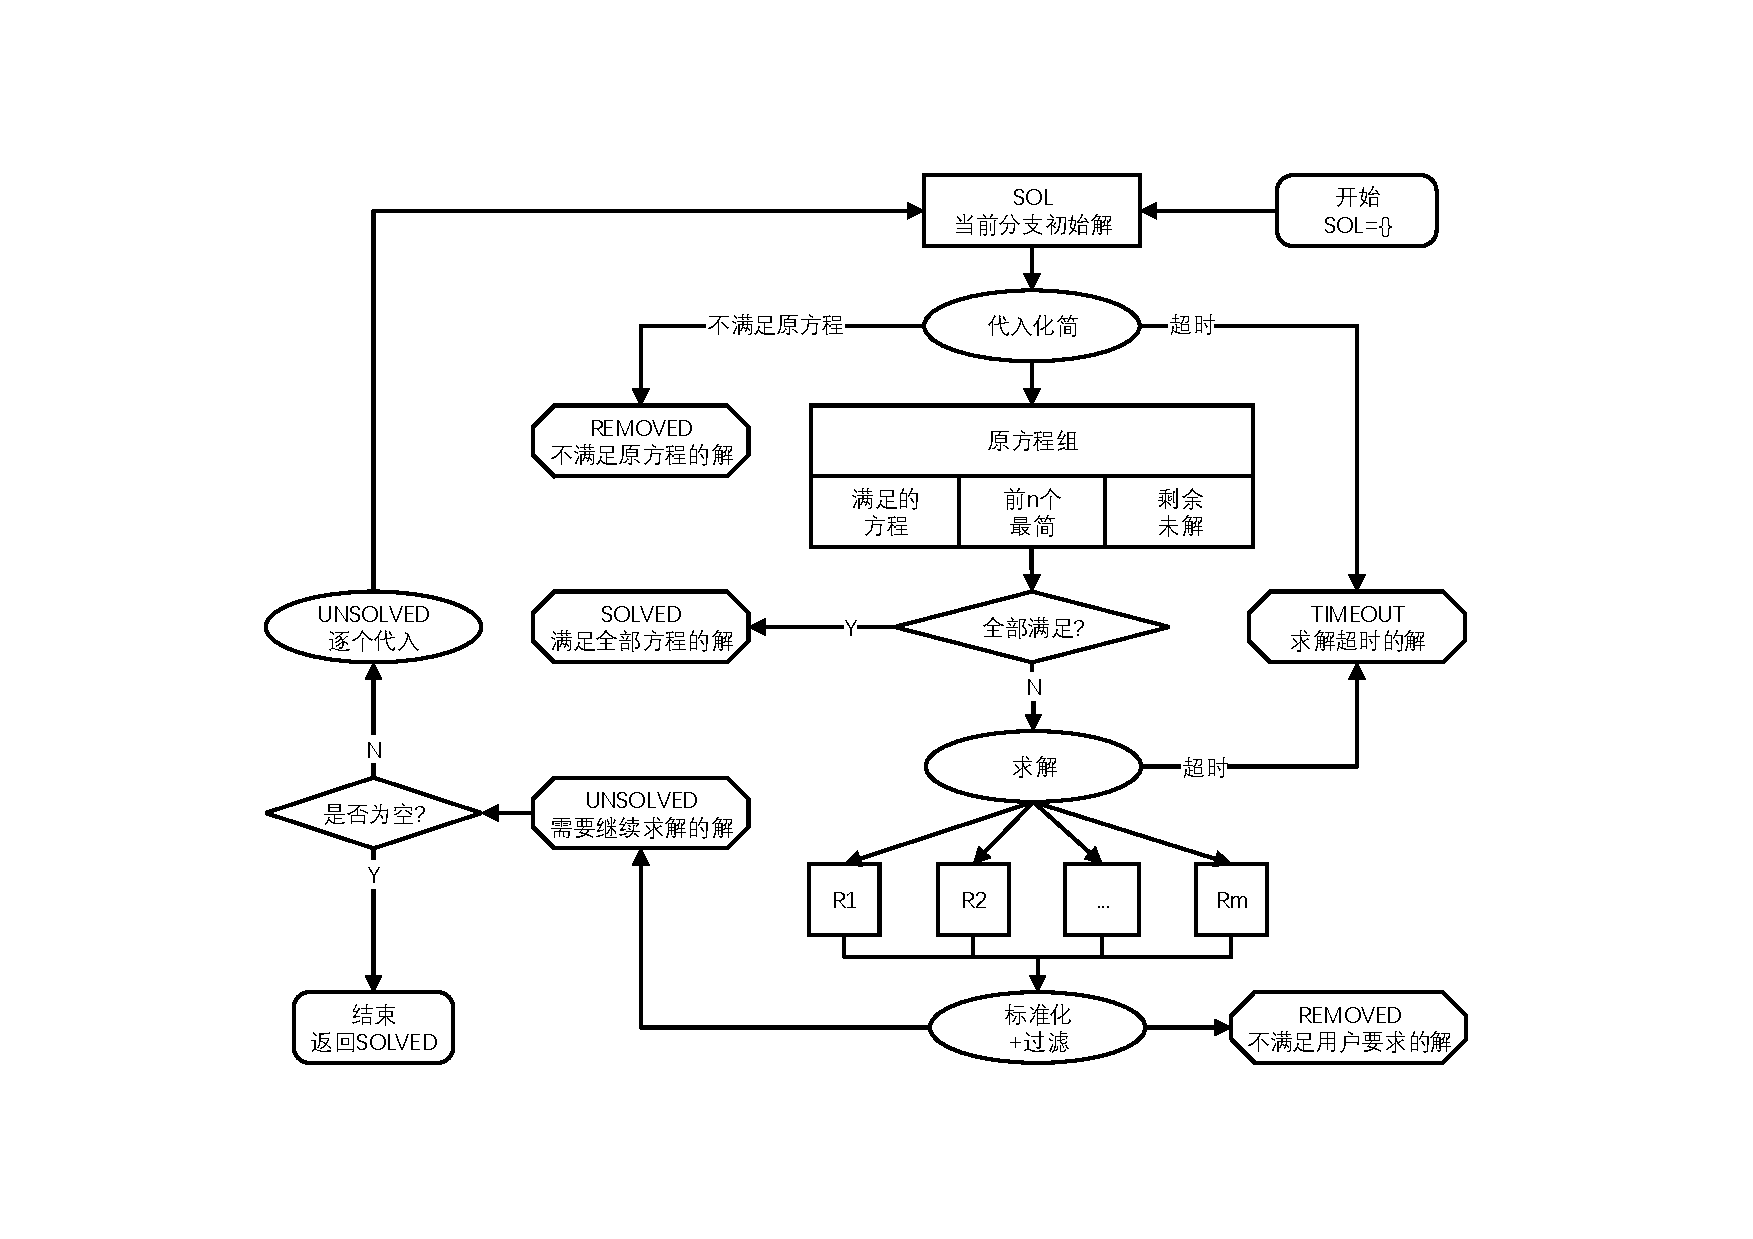
\includegraphics[height=0.8\textheight]{../paper/fig/pgsolve.pdf}
\end{figure}
\end{frame}

\begin{frame}
代入化简所有方程的优势:
\begin{enumerate}
\item 对尚未求解的方程进行代入化简, 能够对新的方程组按照复杂度重新排序, 从而获得更简单的方程.
\item 对已经求解过的方程进行代入化简, 能够验证当前分支的解是否满足这部分方程. 
\item 虽然单个分组只求解了$n$个方程, 但是获得的解可能满足更多的方程, 代入后可以及时地减少待求解方程的数量. 
\end{enumerate}
\end{frame}

\subsection{NS1L: 求n孤子-1 lump相互作用解的软件包}
\begin{frame}
\frametitle{NS1L: 求n孤子-1 lump相互作用解的软件包}
生成公式:
\[
    f_n=\sbrace{\xi_1+\eta_1}^2+\sbrace{\xi_2+\eta_2}^2+\sum_{i=1}^{2^n}\sbrace {q_i\prod_{k \in T_i}{\exp(\xi_{k+2})}}
\]
\[
    \xi_k=\sum_{j=1}^m{p_{j,k}x_j}
\]
约束条件:
\[
\begin{aligned}
    S&=\bbrace{\bbrace{q_i=0}|2\le i \le 2^n} \\ 
        &\cup \bbrace{\bbrace{p_{1,k}=0,\cdots,p_{m,k}=0}|1\le k \le n+2}  \\
        &\cup \bbrace{\bbrace{p_{j,1}=0,p_{j,2}=0}|1\le j \le m} \\ 
        &\cup \bbrace{\bbrace{p_{j,3}=0,\cdots,p_{j,n+2}=0}|1\le j \le m} . 
\end{aligned}
\]
对于一个解$sol$ (是一个集合), 若存在$s\in S$, 满足$s\subseteq sol$, 则$t$就不是我们想要的解.
\end{frame}

\begin{frame}
(3+1)YTSF 方程
\begin{figure}
\centering
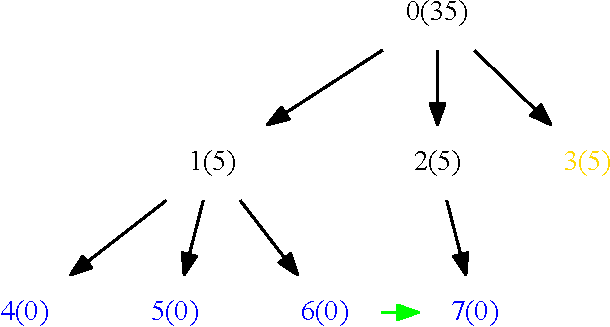
\includegraphics[width=.5\textwidth]{../paper/fig/0S1L.pdf}
\caption{0S-1L 求解分支图 (1秒)}
\end{figure}
\end{frame}

\begin{frame}
\begin{figure}
\centering
\setcounter{subfigure}{0}
\subfigure[]{
    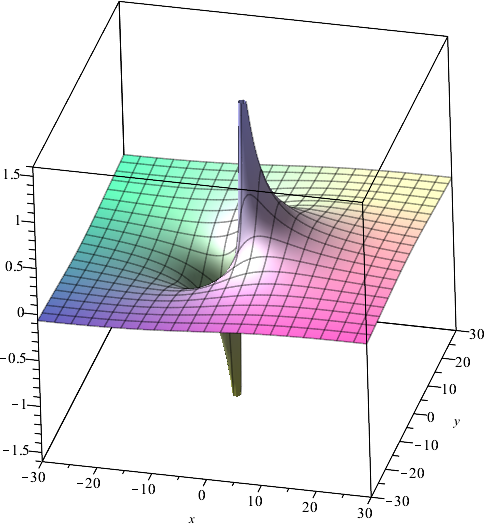
\includegraphics[width=.3\textwidth]{../paper/fig/0S1L-1.png}
}
\subfigure[]{
    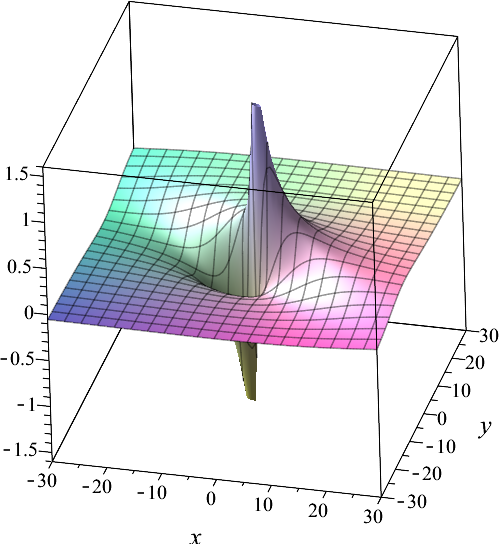
\includegraphics[width=.3\textwidth]{../paper/fig/0S1L-2.png}
}
\caption{(3+1)维 YTSF 方程的 0S-1L 解}
\end{figure}
\end{frame}


\begin{frame}
\begin{figure}
\centering
\setcounter{subfigure}{0}
\subfigure[1S-1L直接求解(8秒)]{
    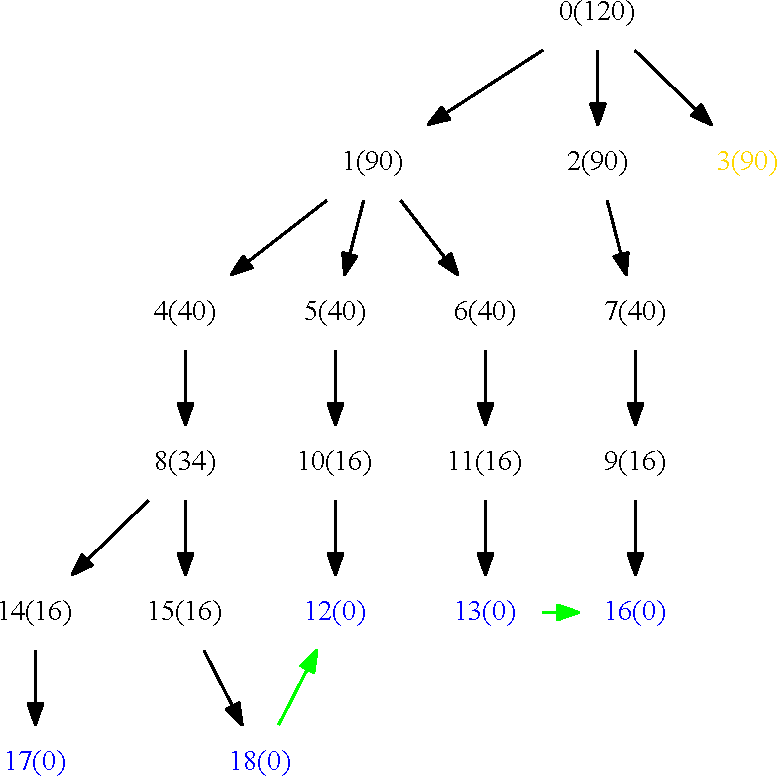
\includegraphics[width=.4\textwidth]{../paper/fig/1S1L-dir.pdf}
}
\hspace{2cm}
\subfigure[1S-1L继承求解(5秒)]{
    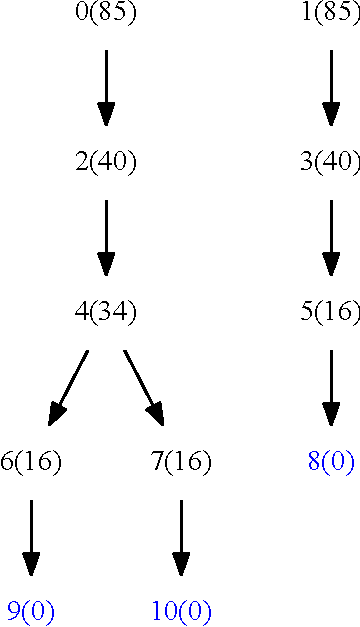
\includegraphics[width=.28\textwidth]{../paper/fig/1S1L-ext.pdf}
}
\end{figure}
\end{frame}

\begin{frame}
\begin{figure}
\centering
\setcounter{subfigure}{0}
\subfigure[]{
    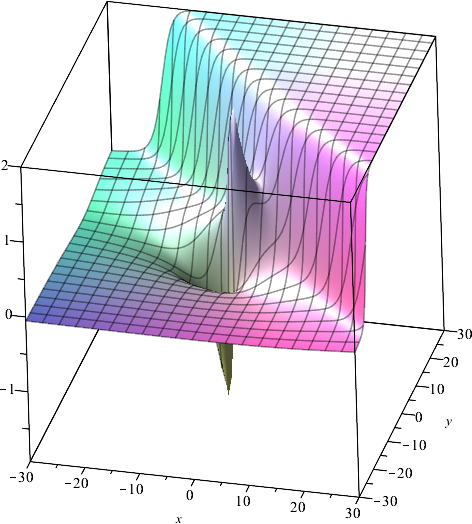
\includegraphics[width=.3\textwidth]{../paper/fig/1S1L-1.png}
}
\subfigure[]{
    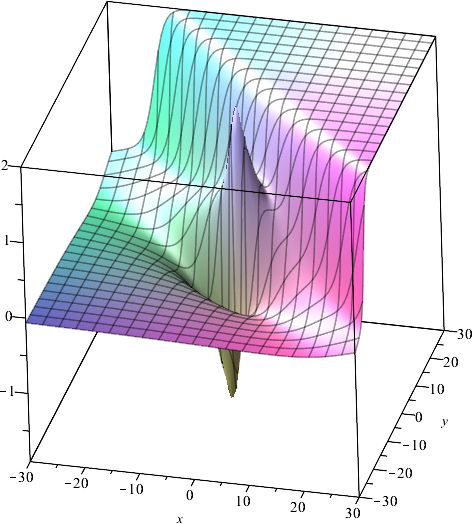
\includegraphics[width=.3\textwidth]{../paper/fig/1S1L-2.png}
}
\subfigure[]{
    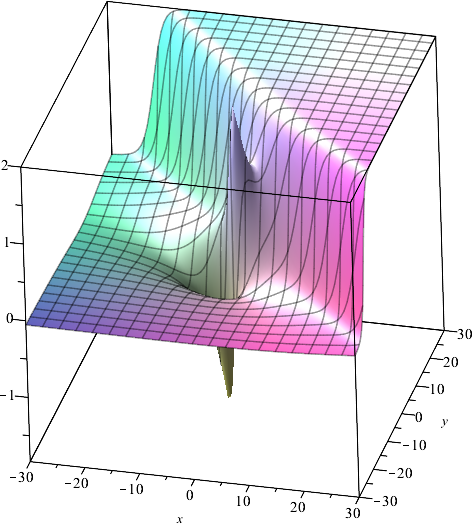
\includegraphics[width=.3\textwidth]{../paper/fig/1S1L-3.png}
}
\caption{(3+1)维 YTSF 方程的 1S-1L 解} \label{fig-1S1L}
\end{figure}
\end{frame}

\frame{
\begin{figure}
\centering
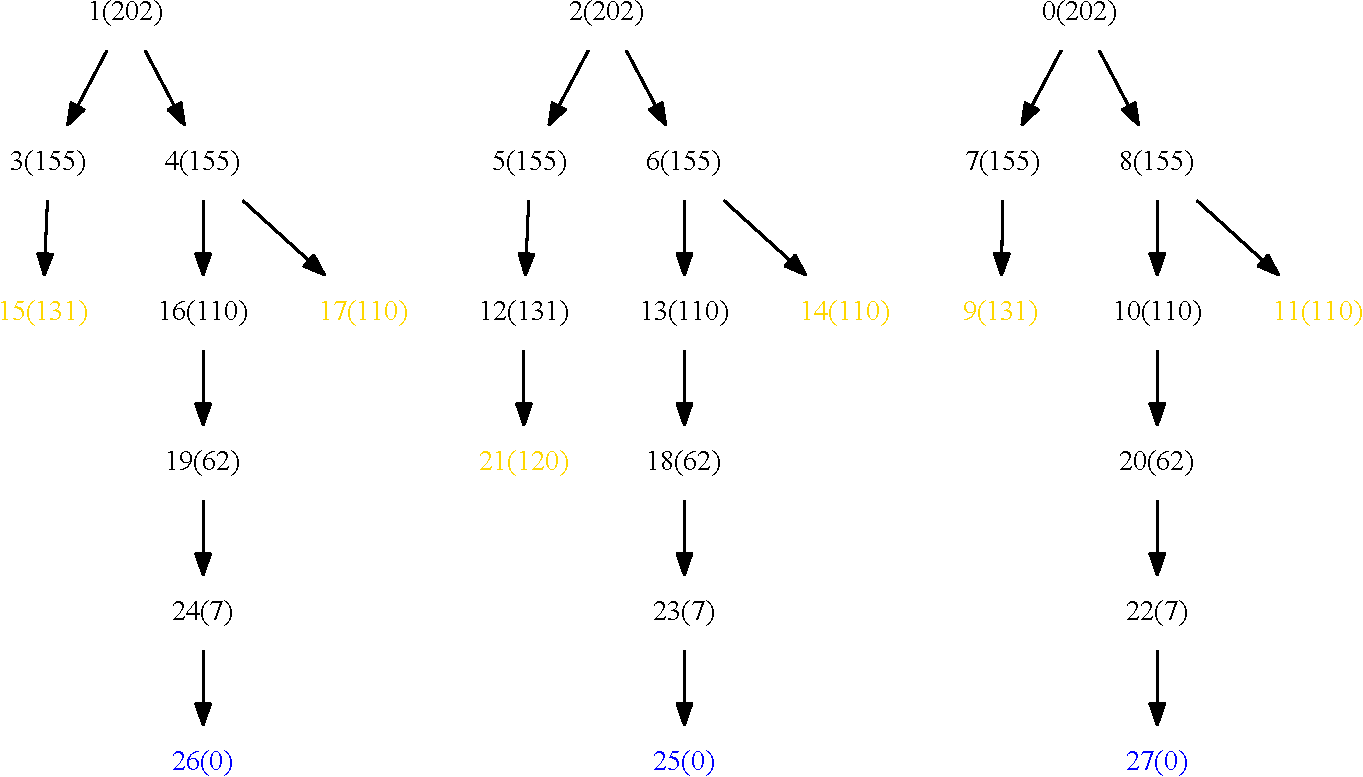
\includegraphics[width=\textwidth]{../paper/fig/2S1L-ext.pdf}
\caption{2S-1L 继承求解的分支图(30 秒)}\label{sb2-e}
\end{figure}
}

\frame{
\begin{figure}
\centering
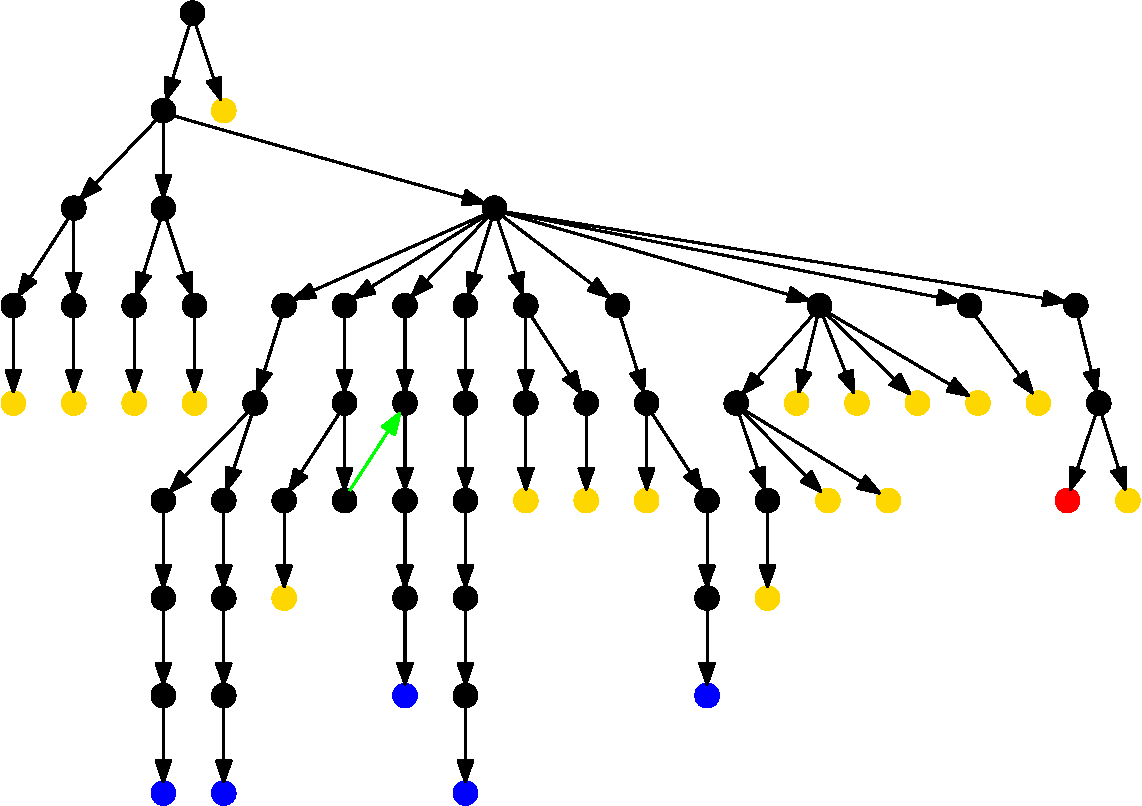
\includegraphics[height=0.8\textheight]{../paper/fig/2S1L-dir-point.pdf}
\caption{2S-1L 直接求解的分支图(430 秒)}\label{sb2-d}
\end{figure}
}

\frame{
\begin{figure}
\centering
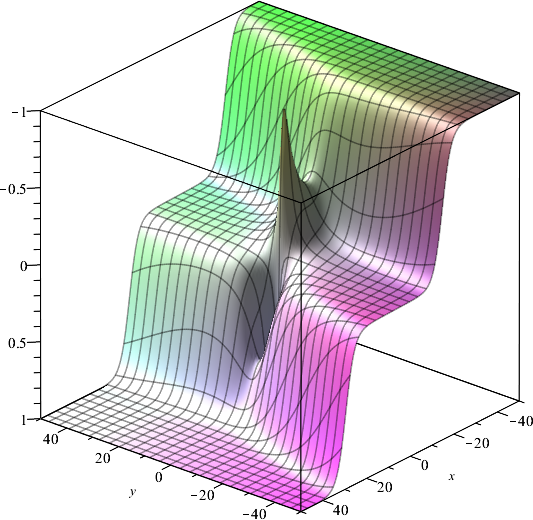
\includegraphics[width=.6\textwidth]{../paper/fig/2S1L.png}
\caption{(3+1)维 YTSF 方程的 2S-1L 解} \label{fig-2S1L}
\end{figure}
}

\subsection{PGSolve 的求解效率}
\begin{frame}
\frametitle{PGSolve 的求解效率}
\begin{adjustbox}{max width=\textwidth}
\centering
\renewcommand{\arraystretch}{1.3}
\begin{tabular}{cccccc}
\hline
来源方程 & 阶数 & 方程数 & 变量数 & PGSolve用时 & Solve用时 \\
\hline
(2+1) SK & 0 & 20 & 9 & 0.724 & 3.483 \\
(2+1) BKP-T & 0 & 20 & 9 & 0.571 & 3.486 \\
(2+1) KP & 0 & 35 & 9 & 1.759 & 29.643 \\
(3+1) YTSF & 0 & 35 & 11 & 1.229 & 8.839 \\
(3+1) JM & 0 & 35 & 11 & 0.845 & >1800 \\
(2+1) SK & 1 & 65 & 13 & 10.241 & >1800 \\
(3+1) YTSF & 1 & 120 & 16 & 12.228 & 1696.852 \\
\hline
\end{tabular}
\end{adjustbox}

\vspace{1em}

此处对比的是\cd{PDEtools:-Solve}. 而最常用的\cd{solve}函数甚至不能在 72 小时内求解只有 20 个方程的方程组, 这显然是\cd{solve}函数的一个 BUG.

\end{frame}

\begin{frame}

\begin{adjustbox}{max width=\textwidth}
\renewcommand{\arraystretch}{1.3}
\begin{tabular}{cccccc}
\hline
方程名称    & 解的阶数 & 方程数量 & 分组大小 & 解的个数 & 运行时间(s) \\ 
\hline 
(2+1)SK & 0 & 20 & 5 & 1 & 2.197 \\
(2+1)SK & 1 & 65 & 3 & 1 & 3.072 \\
(2+1)SK & 2 & 179 & 5 & 2 & 12.697 \\
(2+1)BKP-T & 0 & 20 & 5 & 1 & 1.036 \\
(2+1)BKP-T & 1 & 65 & 3 & 1 & 3.251 \\
(2+1)BKP-T & 2 & 179 & 5 & 2 & 12.617 \\
(3+1)YTSF & 0 & 35 & 5 & 2 & 1.948 \\
(3+1)YTSF & 1 & 120 & 5 & 3 & 6.717 \\
(3+1)YTSF & 2 & 324 & 5 & 3 & 37.909 \\
(3+1)JM & 0 & 35 & 5 & 3 & 2.014 \\
(3+1)JM & 1 & 120 & 5 & 13 & 18.384 \\
(3+1)JM & 2 & 324 & 5 & 4 & 50.934 \\
\hline 
\end{tabular}
\end{adjustbox}

\end{frame}